\subsection{Experimental setup}
\label{sec:setup}

\subsubsection{System}
\label{sec:system}

For our experiments, we use a server that has an x86-based 64-bit AMD EPYC-7742 processor. This processor has a clock frequency of $2.25$ GHz and $512$ GB of DDR4 system memory. Each core has an L1 cache of $4$ MB, an L2 cache of $32$ MB, and a shared L3 cache of $256$ MB. The machine uses Ubuntu 20.04.


\subsubsection{Configuration}
\label{sec:configuration}

We use 32-bit unsigned integer for vertex IDs, 32-bit floating point for edge weights, but use 64-bit floating point for hashtable values, total edge weight, modularity calculation, and all places where performing an aggregation/sum of floating point values. Affected vertices are represented with an 8-bit integer vector. Computing the weighted degree of each vertex, the local moving phase, and aggregating the edges for the super-vertex graph, employ OpenMP's \textit{dynamic schedule} with a chunk size of $2048$ for dynamic workload balancing among threads. We set the iteration tolerance $\tau$ to $10^{-2}$, the tolerance drop per pass $TOLERANCE\_DECLINE\_FACTOR$ to $10$ (threshold-scaling optimization), maximum number of iterations per pass $MAX\_ITERATI$ $ONS$ to $20$, and the maximum number of passes $MAX\_PASSES$ to $10$. Further, we set the aggregation tolerance $\tau_{agg}$ to $0.8$ for large (static) graphs with generated random batch updates, but keep it disabled, i.e., set $\tau_{agg}$ to $1$, for real-world dynamic graphs. Unless mentioned otherwise, we execute all parallel implementations with a default of $64$ threads (to match the number of cores available on the system). We use GCC 9.4 and OpenMP 5.0 \cite{openmp18} for compilation.


\subsubsection{Dataset}
\label{sec:dataset}

To experiment with real-world dynamic graphs, we employ five temporal networks sourced from the Stanford Large Network Dataset Collection \cite{snapnets}, detailed in Table \ref{tab:dataset}. Here, the number of vertices range from $24.8$ thousand to $2.60$ million, temporal edges from $507$ thousand to $63.4$ million, and static edges from $240$ thousand to $36.2$ million. For experiments involving large static graphs with random batch updates, we utilize $12$ graphs as listed in Table \ref{tab:dataset-large}, obtained from the SuiteSparse Matrix Collection \cite{suite19}. Here, the number of vertices in the graphs varies from $3.07$ to $214$ million, and the number of edges varies from $25.4$ million to $3.80$ billion. With each graph, we ensure that all edges are undirected and weighted with a default weight of $1$.

\begin{table}[hbtp]
  \centering
  \caption{List of $5$ real-world dynamic graphs\ignore{, i.e., temporal networks}, sourced from the Stanford Large Network Dataset Collection \cite{snapnets}. Here, $|V|$ denotes the number of vertices, $|E_T|$ represents the count of temporal edges (inclusive of duplicates), and $|E|$ indicates the number of static edges (without duplicates).}
  \label{tab:dataset}
  \begin{tabular}{|c||c|c|c|c|}
    \toprule
    \textbf{Graph} &
    \textbf{\textbf{$|V|$}} &
    \textbf{\textbf{$|E_T|$}} &
    \textbf{\textbf{$|E|$}} \\
    \midrule
    sx-mathoverflow & 24.8K & 507K & 240K \\ \hline
    sx-askubuntu & 159K & 964K & 597K \\ \hline
    sx-superuser & 194K & 1.44M & 925K \\ \hline
    wiki-talk-temporal & 1.14M & 7.83M & 3.31M \\ \hline
    sx-stackoverflow & 2.60M & 63.4M & 36.2M \\ \hline
  \bottomrule
  \end{tabular}
\end{table}

\begin{table}[hbtp]
  \centering
  \caption{List of $12$ graphs retrieved from the SuiteSparse Matrix Collection \cite{suite19} (with directed graphs indicated by $*$). Here, $|V|$ denotes the number of vertices, $|E|$ denotes the number of edges (after making the graph undirected by adding reverse edges), and $|\Gamma|$ denotes the number of communities obtained with \textit{Static Leiden} algorithm \cite{sahu2023gveleiden}.}
  \label{tab:dataset-large}
  \begin{tabular}{|c||c|c|c|}
    \toprule
    \textbf{Graph} &
    \textbf{\textbf{$|V|$}} &
    \textbf{\textbf{$|E|$}} &
    \textbf{\textbf{$|\Gamma|$}} \\
    \midrule
    \multicolumn{4}{|c|}{\textbf{Web Graphs (LAW)}} \\ \hline
    indochina-2004$^*$ & 7.41M & 341M & 2.68K \\ \hline
    arabic-2005$^*$ & 22.7M & 1.21B & 2.92K \\ \hline
    uk-2005$^*$ & 39.5M & 1.73B & 18.2K \\ \hline
    webbase-2001$^*$ & 118M & 1.89B & 2.94M \\ \hline
    it-2004$^*$ & 41.3M & 2.19B & 4.05K \\ \hline
    sk-2005$^*$ & 50.6M & 3.80B & 2.67K \\ \hline
    \multicolumn{4}{|c|}{\textbf{Social Networks (SNAP)}} \\ \hline
    com-LiveJournal & 4.00M & 69.4M & 3.09K \\ \hline
    com-Orkut & 3.07M & 234M & 36 \\ \hline
    \multicolumn{4}{|c|}{\textbf{Road Networks (DIMACS10)}} \\ \hline
    asia\_osm & 12.0M & 25.4M & 2.70K \\ \hline
    europe\_osm & 50.9M & 108M & 6.13K \\ \hline
    \multicolumn{4}{|c|}{\textbf{Protein k-mer Graphs (GenBank)}} \\ \hline
    kmer\_A2a & 171M & 361M & 21.1K \\ \hline
    kmer\_V1r & 214M & 465M & 10.5K \\ \hline
  \bottomrule
  \end{tabular}
\end{table}



\subsubsection{Batch generation}
\label{sec:batch-generation}

For experiments involving real-world dynamic graphs, we first load $90\%$ of each graph from Table \ref{tab:dataset}, and ensure that all edges are weigthed with a default weight of $1$, and that they are undirected by adding the reverse edges. Subsequently, we load $B$ edges in $100$ batch updates. Here, $B$ denotes the desired batch size, specified as a fraction of the total number of temporal edges $|E_T|$ in the graph, and ensure that the batch update is undirected. For experiments on large graphs with random batch updates, we take each base graph from Table \ref{tab:dataset-large} and generate random batch updates \cite{com-zarayeneh21} comprising an $80\% : 20\%$ mix of edge insertions and deletions to emulate realistic batch updates, each with an edge weight of $1$. To prepare the set of edges for insertion, we select vertex pairs with equal probability. For edge deletions, we uniformly delete each existing edge. To simplify, we ensure no new vertices are added or removed from the graph. The batch size is measured as a fraction of edges in the original graph, ranging from $10^{-7}$ to $0.1$ (i.e., $10^{-7}|E|$ to $0.1|E|$), with multiple batches generated for each size for averaging. For a billion-edge graph, this amounts to a batch size of $100$ to $100$ million edges.\ignore{Keep in mind that dynamic graph algorithms are helpful for small batch sizes in interactive applications. For large batches, it is usually more efficient to run the static algorithm.} All batch updates are undirected, i.e., for every edge insertion $(i, j, w)$ in the batch update, the edge $(j, i, w)$ is also a part of the batch update. We employ five distinct random batch updates for each batch size, and report average across these runs in our experiments.


\subsubsection{Measurement}
\label{sec:measurement}

We evaluate the runtime of each approach on the entire updated graph, including the local-moving phase, aggregation phase, the initial and incremental marking of affected vertices, convergence detection, and all the necessary intermediary steps, but excluding memory allocation/deallocation time. We assume that the total edge weight of the graphs is known, and can be tracked upon each batch update.

\begin{figure*}[!hbt]
  \centering
  \subfigure[Overall Runtime]{
    \label{fig:temporal-summary--runtime-overall}
    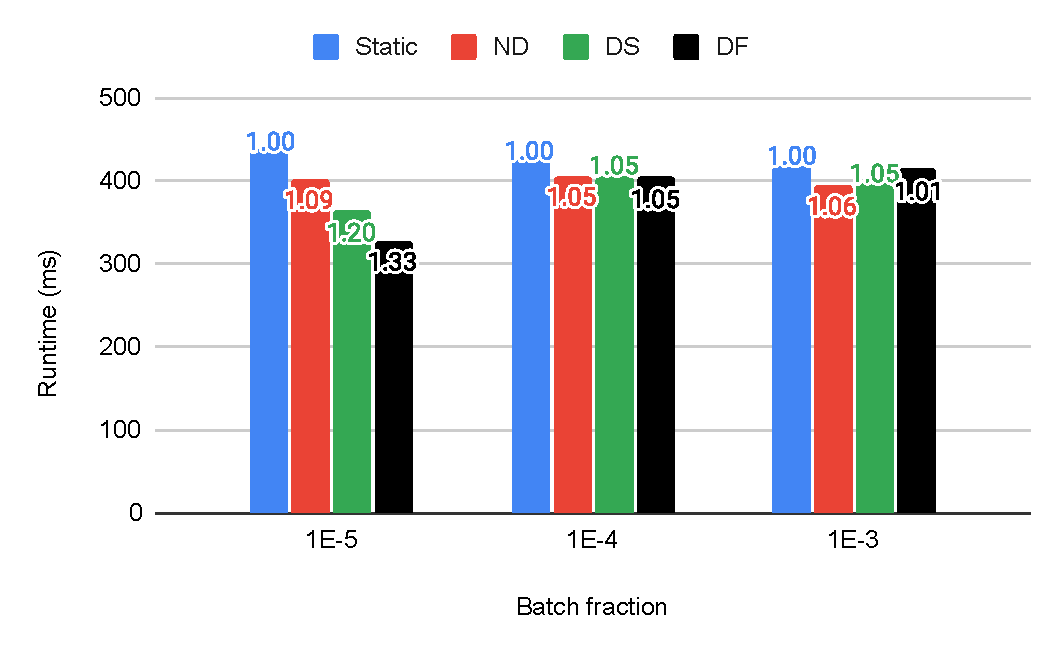
\includegraphics[width=0.48\linewidth]{out/temporal-summary-runtime-overall.pdf}
  }
  \subfigure[Overall Modularity of communities obtained]{
    \label{fig:temporal-summary--modularity-overall}
    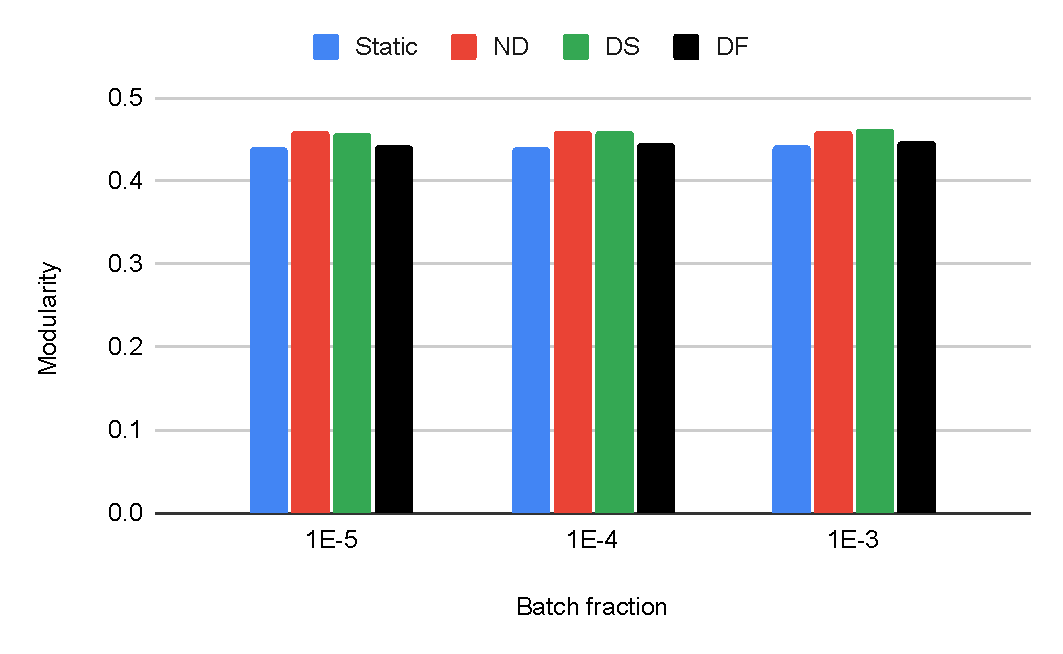
\includegraphics[width=0.48\linewidth]{out/temporal-summary-modularity-overall.pdf}
  } \\[2ex]
  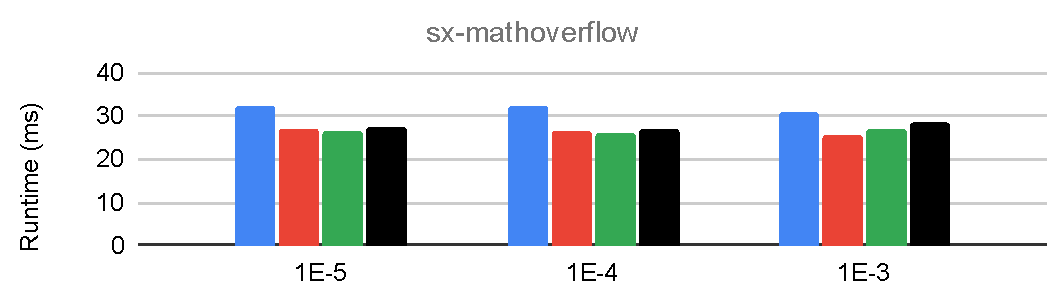
\includegraphics[width=0.48\linewidth]{out/temporal-summary-runtime-sx-mathoverflow.pdf}
  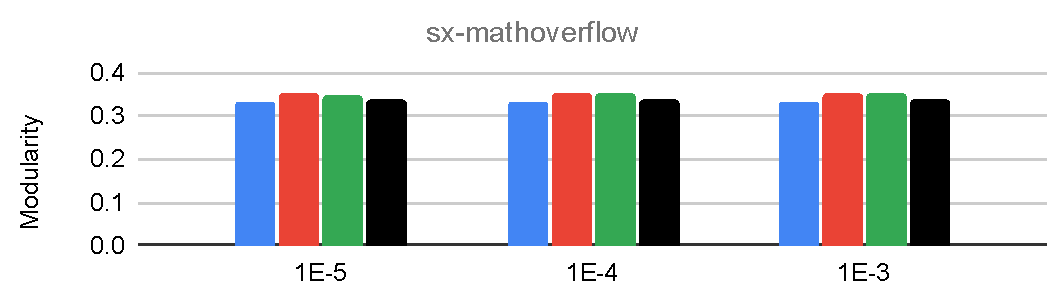
\includegraphics[width=0.48\linewidth]{out/temporal-summary-modularity-sx-mathoverflow.pdf}
  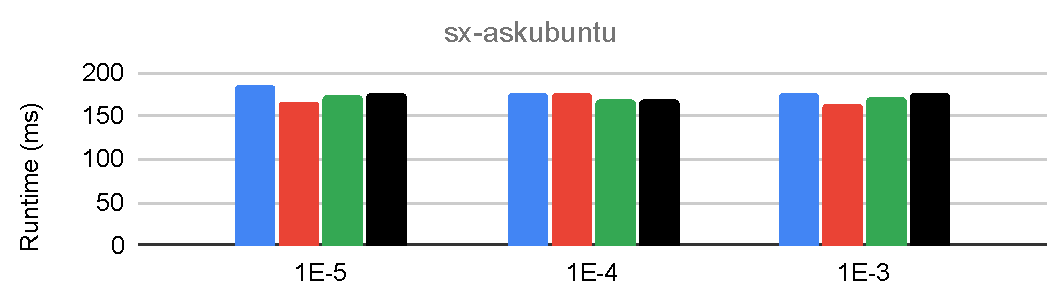
\includegraphics[width=0.48\linewidth]{out/temporal-summary-runtime-sx-askubuntu.pdf}
  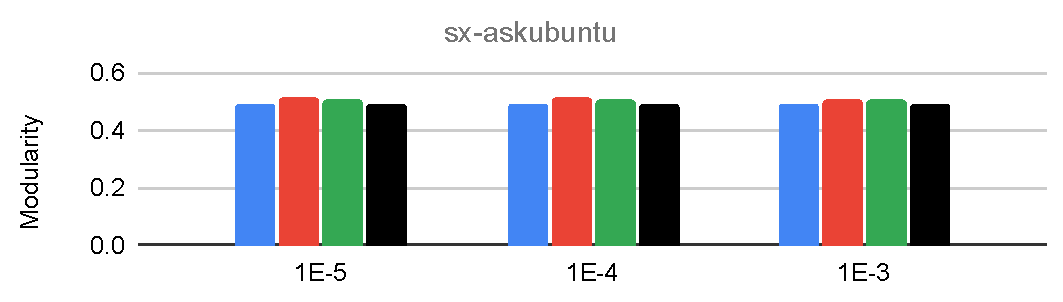
\includegraphics[width=0.48\linewidth]{out/temporal-summary-modularity-sx-askubuntu.pdf}
  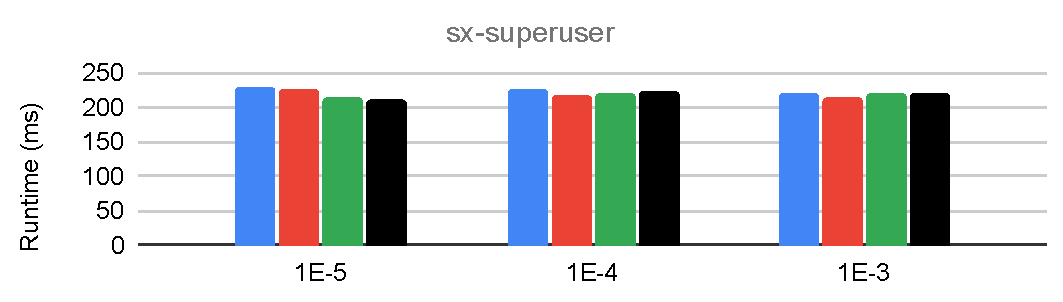
\includegraphics[width=0.48\linewidth]{out/temporal-summary-runtime-sx-superuser.pdf}
  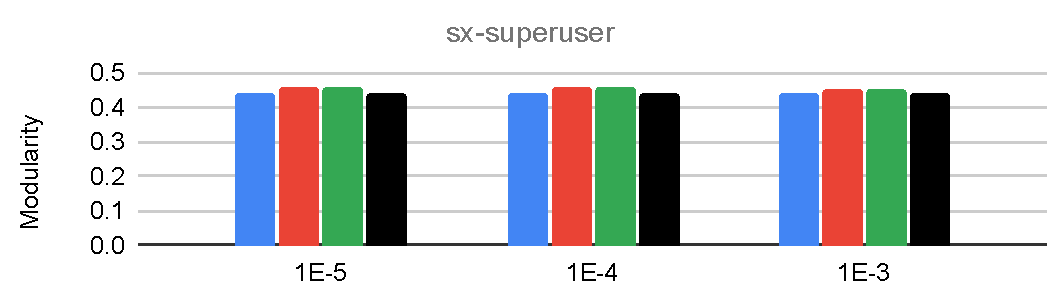
\includegraphics[width=0.48\linewidth]{out/temporal-summary-modularity-sx-superuser.pdf}
  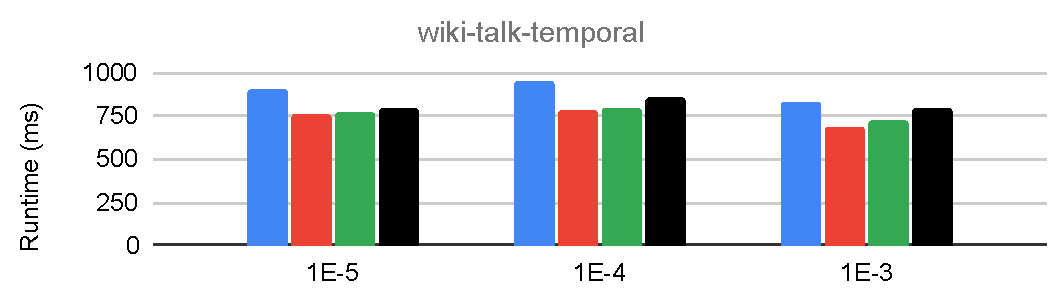
\includegraphics[width=0.48\linewidth]{out/temporal-summary-runtime-wiki-talk-temporal.pdf}
  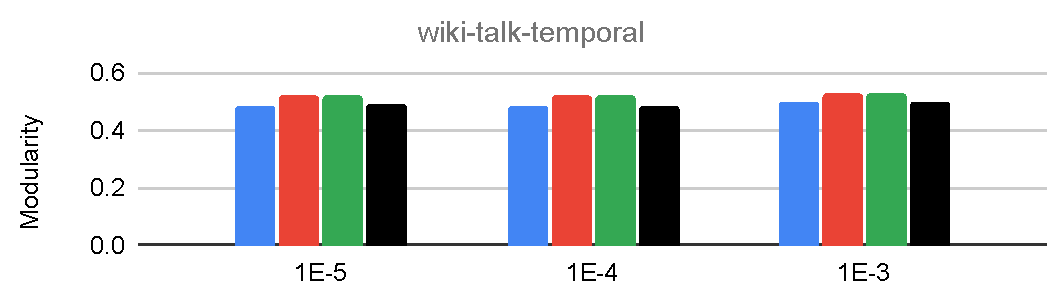
\includegraphics[width=0.48\linewidth]{out/temporal-summary-modularity-wiki-talk-temporal.pdf}
  \subfigure[Runtime on each dynamic graph]{
    \label{fig:temporal-summary--runtime-graph}
    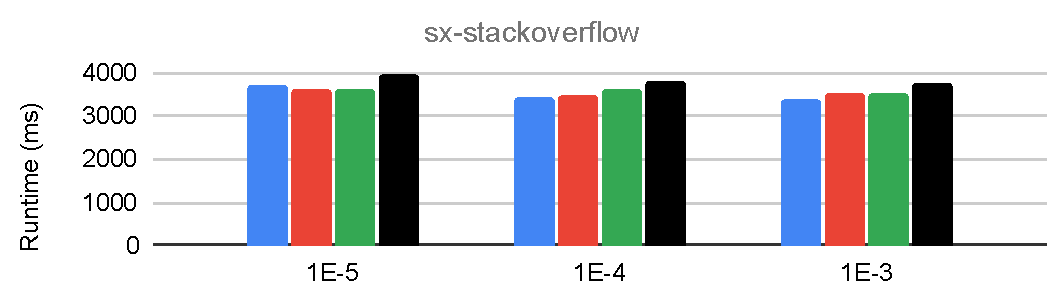
\includegraphics[width=0.48\linewidth]{out/temporal-summary-runtime-sx-stackoverflow.pdf}
  }
  \subfigure[Modularity in communities obtained on each dynamic graph]{
    \label{fig:temporal-summary--modularity-graph}
    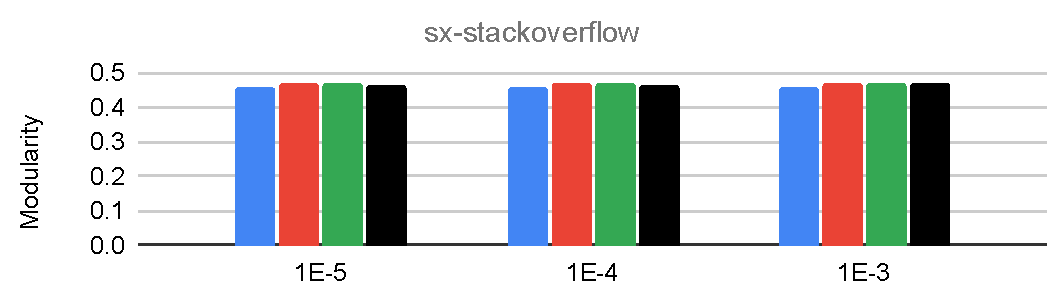
\includegraphics[width=0.48\linewidth]{out/temporal-summary-modularity-sx-stackoverflow.pdf}
  } \\[-2ex]
  \caption{Mean Runtime and Modularity of communities obtained with our multicore implementation of \textit{Static}, \textit{Naive-dynamic (ND)}, \textit{Delta-screening (DS)}, and \textit{Dynamic Frontier (DF)} Leiden on real-world dynamic graphs, with batch updates of size $10^{-5}|E_T|$ to $10^{-3}|E_T|$. Here, (a) and (b) show the overall runtime and modularity across all temporal graphs, while (c) and (d) show the runtime and modularity for each graph. In (a), the speedup of each approach with respect to Static Leiden is labeled.}
  \label{fig:temporal-summary}
\end{figure*}

\begin{figure*}[hbtp]
  \centering
  \subfigure[Overall result]{
    \label{fig:8020-runtime--mean}
    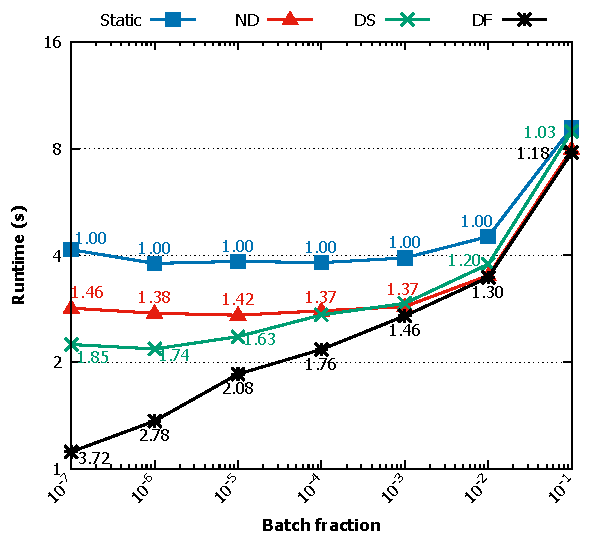
\includegraphics[width=0.38\linewidth]{out/8020-runtime-mean.pdf}
  }
  \subfigure[Results on each graph]{
    \label{fig:8020-runtime--all}
    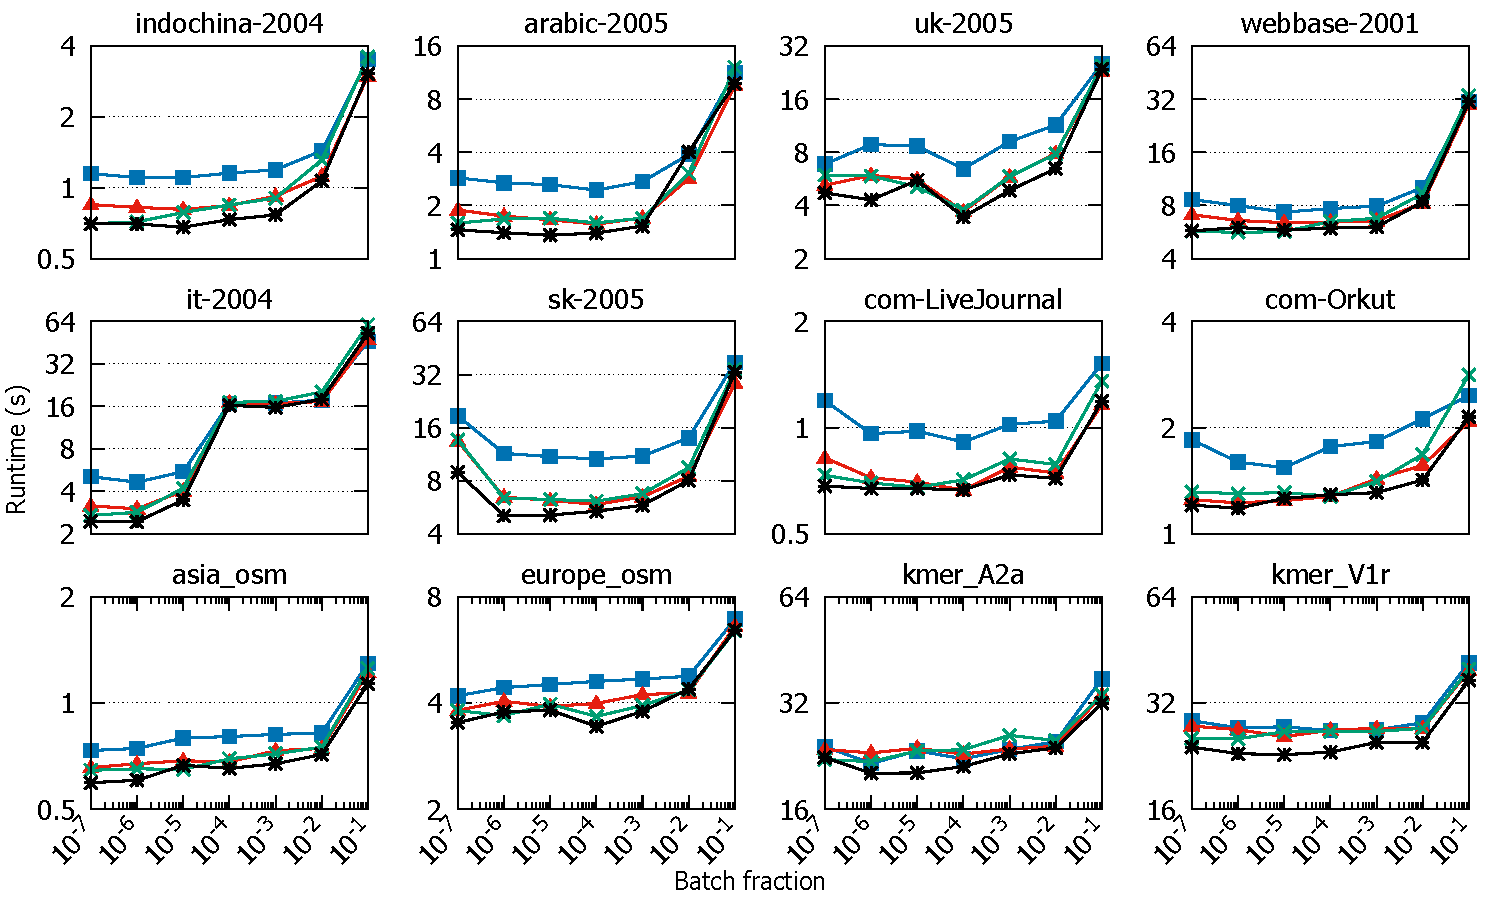
\includegraphics[width=0.58\linewidth]{out/8020-runtime-all.pdf}
  } \\[0ex]
  \caption{Runtime (logarithmic scale) of our multicore implementation of \textit{Naive-dynamic (ND)}, \textit{Delta-screening (DS)}, and \textit{Dynamic Frontier (DF) Leiden}, compared to \textit{Static Leiden} \cite{sahu2024fast}, on large\ignore{(static)} graphs with randomly generated batch updates. The size of these batch updates ranges from $10^{-7}|E|$ to $0.1|E|$ in multiples of $10$, with the updates comprising $80\%$ edge insertions and $20\%$ edge deletions to simulate realistic dynamic graph changes. The right subfigure shows the runtime of each algorithm for individual graphs in the dataset, while the left subfigure displays overall runtimes using the geometric mean for consistent scaling across graphs.\ignore{Furthermore,} The speedup of each algorithm compared to Static Leiden is indicated on the respective lines.}
  \label{fig:8020-runtime}
\end{figure*}

\begin{figure*}[hbtp]
  \centering
  \subfigure[Overall result]{
    \label{fig:8020-modularity--mean}
    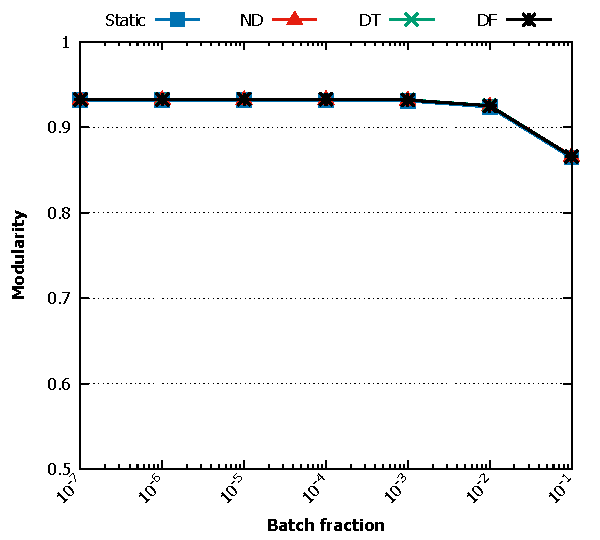
\includegraphics[width=0.38\linewidth]{out/8020-modularity-mean.pdf}
  }
  \subfigure[Results on each graph]{
    \label{fig:8020-modularity--all}
    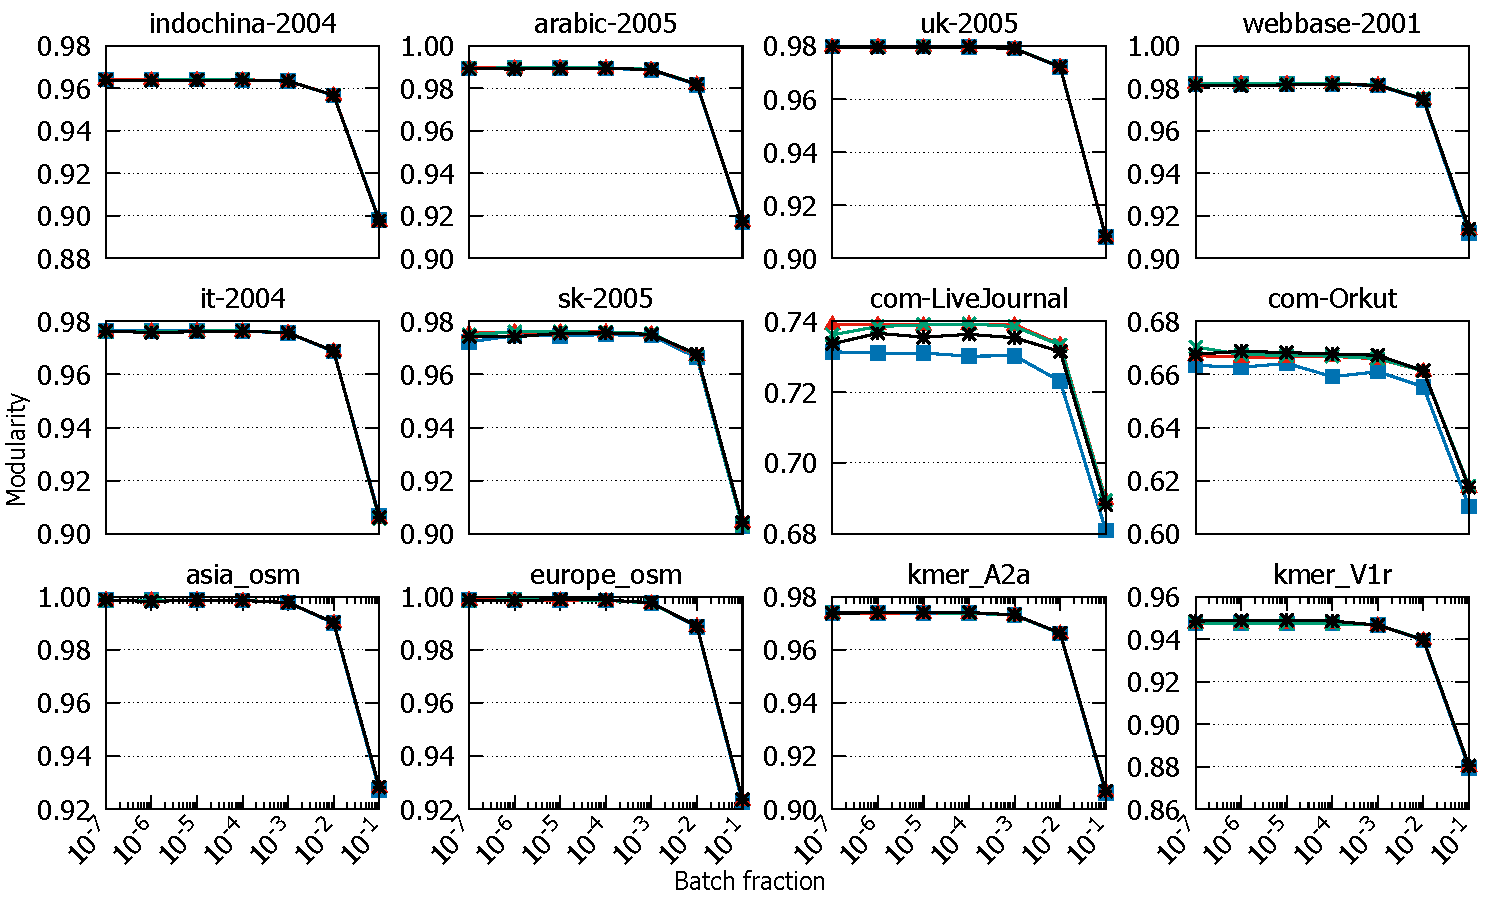
\includegraphics[width=0.58\linewidth]{out/8020-modularity-all.pdf}
  } \\[-2ex]
  \caption{Modularity comparison of our multicore implementation of \textit{Static}, \textit{Naive-dynamic (ND)}, \textit{Delta-screening (DS)}, and \textit{Dynamic Frontier (DF)} Leiden on large (static) graphs with generated random batch updates. The size of batch updates range from $10^{-7} |E|$ to $0.1 |E|$ in multiples of $10$ (logarithmic scale), consisting of $80\%$ edge insertions and $20\%$ edge deletions to simulate realistic dynamic graph updates. The right subfigure depicts the modularity for each approach in relation to each graph, while the left subfigure showcases overall modularity using arithmetic mean.}
  \label{fig:8020-modularity}
\end{figure*}





\subsection{Performance Comparison}
\label{sec:performance-comparison}

\subsubsection{Results on real-world dynamic graphs}

We now compare the performance of our Parallel Dynamic Frontier (DF) Leiden with our parallel implementation of Static, Naive-dynamic (ND), and Delta-screening (DS) Leiden on real-world dynamic graphs from Table \ref{tab:dataset}. These evaluations are conducted on batch updates of size $10^{-5}|E_T|$ to $10^{-3}|E_T|$ in multiples of $10$. For each batch size, as mentioned in Section \ref{sec:batch-generation}, we load $90\%$ of the graph, add reverse edges to make all edges in the graph undirected, and then load $B$ edges (where $B$ is the batch size) consecutively in $100$ batch updates. The work of Zarayeneh et al. \cite{com-zarayeneh21} demonstrates improved performance of the DS approach compared to DynaMo \cite{com-zhuang19} and Batch \cite{com-chong13}. Thus, we limit our comparison to DS Leiden. Figure \ref{fig:temporal-summary--runtime-overall} displays the overall runtime of each approach across all graphs for each batch size, while Figure \ref{fig:temporal-summary--modularity-overall} illustrates the overall modularity of obtained communities. Additionally, Figures \ref{fig:temporal-summary--runtime-graph} and \ref{fig:temporal-summary--modularity-graph} present the mean runtime and modularity of communities obtained with the approaches on each dynamic graph in the dataset.

Figure \ref{fig:temporal-summary--runtime-overall} shows that DF Leiden is, on average, $268\times$, $195\times$, and $109\times$ faster than Static Leiden on batch updates of size $10^{-5}|E_T|$, $10^{-4}|E_T|$, and $10^{-3}|E_T|$, respectively. In contrast, DS Leiden demonstrates average speedups of $47\times$, $32\times$, and $26\times$ over Static Leiden for batch update sizes of $10^{-5}|E_T|$ to $10^{-3}|E_T|$, while ND Leiden obtains a mean speedup of $25\times$\ignore{over Static Leiden}.\ignore{DF Leiden thus achieves average speedups of $5.7\times$, $6.1\times$, and $4.2\times$ compared to DS Leiden for the same batch updates.} DF Leiden is thus, overall, $179\times$, $7.2\times$, and $5.3\times$ faster than Static, ND, and DS Leiden. This speedup is particularly pronounced on the \textit{sx-superuser} graph, as indicated by Figure \ref{fig:temporal-summary--runtime-graph}. Regarding modularity, Figures \ref{fig:temporal-summary--modularity-overall} and \ref{fig:temporal-summary--modularity-graph} illustrate that DF Leiden generally exhibits slightly lower modularity on average compared to ND and DS Leiden but is on par with the modularity obtained by Static Leiden, except for the \textit{sx-superuser} graph (because it fails to mark certain vertices as affected, likely because they are outlier vertices and were not directly reached from the expanding frontier). This makes the communities obtained with DF Leiden generally acceptable. However, if lower modularity is observed (during intermediate empirical tests), transitioning to our parallel implementation of DS Leiden is advisable.


\subsubsection{Results on large graphs with random batch updates}

We also assess the performance of our parallel DF Leiden alongside our parallel implementation of Static, ND, and DS Leiden on large (static) graphs listed in Table \ref{tab:dataset-large}, with randomly generated batch updates. As elaborated in Section \ref{sec:batch-generation}, the batch updates vary in size from $10^{-7}|E|$ to $0.1|E|$ (in multiples of $10$), comprising $80\%$ edge insertions and $20\%$ edge deletions to mimic realistic scenarios. Reverse edges are added with each batch update, to ensure that the graph is undirected. As mentioned in Section \ref{sec:batch-generation}, we generate $5$ different random batch updates for each batch size to minimize measurement noise. Figure \ref{fig:8020-runtime} illustrates the runtime of Static, ND, DS, and DF Leiden, while Figure \ref{fig:8020-modularity} displays the modularity of communities obtained with each approach.

Figure \ref{fig:8020-runtime--mean} illustrates that DF Leiden achieves a mean speedup of $183\times$, $13.8\times$, and $8.7\times$ compared to Static, ND, and DS Leiden, respectively. On a batch update of size $10^{-7}|E|$, DF Leiden is significantly faster, attaining speedups of $540\times$, $39\times$, and $14\times$, with respect to Static, ND, and DS Leiden, respectively. The speedup is particularly pronounced on web graphs, social networks, and protein k-mer graphs, characterized by a large number of vertices (as depicted in Figure \ref{fig:8020-runtime--all}). It may be noted that DS Leiden exhibits slower performance than ND Leiden on large batch updates, i.e., on batch updates of size $0.01|E|$ and $0.1|E|$. This is attributed to the cost of initial marking of affected vertices with DS Leiden --- since the updates are scattered randomly across the graph, DS Leiden ends up marking a significant number of vertices as affected, making it almost equivalent to ND Leiden, but with the added cost of the marking of affected vertices (particularly on web graphs and social networks, characterized by a high average degree and a small diameter). Figures \ref{fig:8020-modularity--mean} and \ref{fig:8020-modularity--all} indicate that DF Leiden obtains communities with the roughly same modularity as Static, ND, and DS Leiden. Hence, for large graphs with random batch updates, DF Leiden is the best dynamic community detection method.

In Figure \ref{fig:8020-runtime}, also note that runtime of Static Leiden increases for larger batch updates. This more likely due to the random batch updates arbitrarily disrupting the original community structure --- which results in Static Leiden needing more iterations to converge --- than due to the increased number of edges in the graph.
